\section{Expected Benefits, Limitations and Examples of Intelligent Textbook Integration}
\label{sec:benefits}
\label{sec:limitations}

\subsection{Introduction: Research Foundation for Interactive Simulations}

Educational research consistently demonstrates the effectiveness of interactive simulations for enhancing learning outcomes across STEM disciplines. Meta-analyses and systematic reviews provide compelling evidence that well-designed simulations significantly improve student engagement, conceptual understanding, and long-term knowledge retention \cite{wieman2008phet, rutten2012learning, dangelo2014simulations}. This substantial body of research, accumulated over decades of classroom implementation and controlled studies, establishes interactive simulations as transformative pedagogical tools that address persistent challenges in STEM education.

Studies consistently report that students using interactive simulations exhibit higher interest and participation in STEM lessons, with measurable improvements in both immediate learning outcomes and sustained understanding. Meta-analyses across STEM disciplines demonstrate that students using interactive simulations consistently outperform peers receiving traditional instruction alone:

\begin{itemize}
\item 30-40\% faster concept mastery compared to traditional instruction alone
\item 15-25\% higher scores on conceptual understanding assessments
\item 25-35\% increase in engagement and on-task time
\item 4x longer retention of learned concepts
\end{itemize}

\begin{figure}[htbp]
\centering
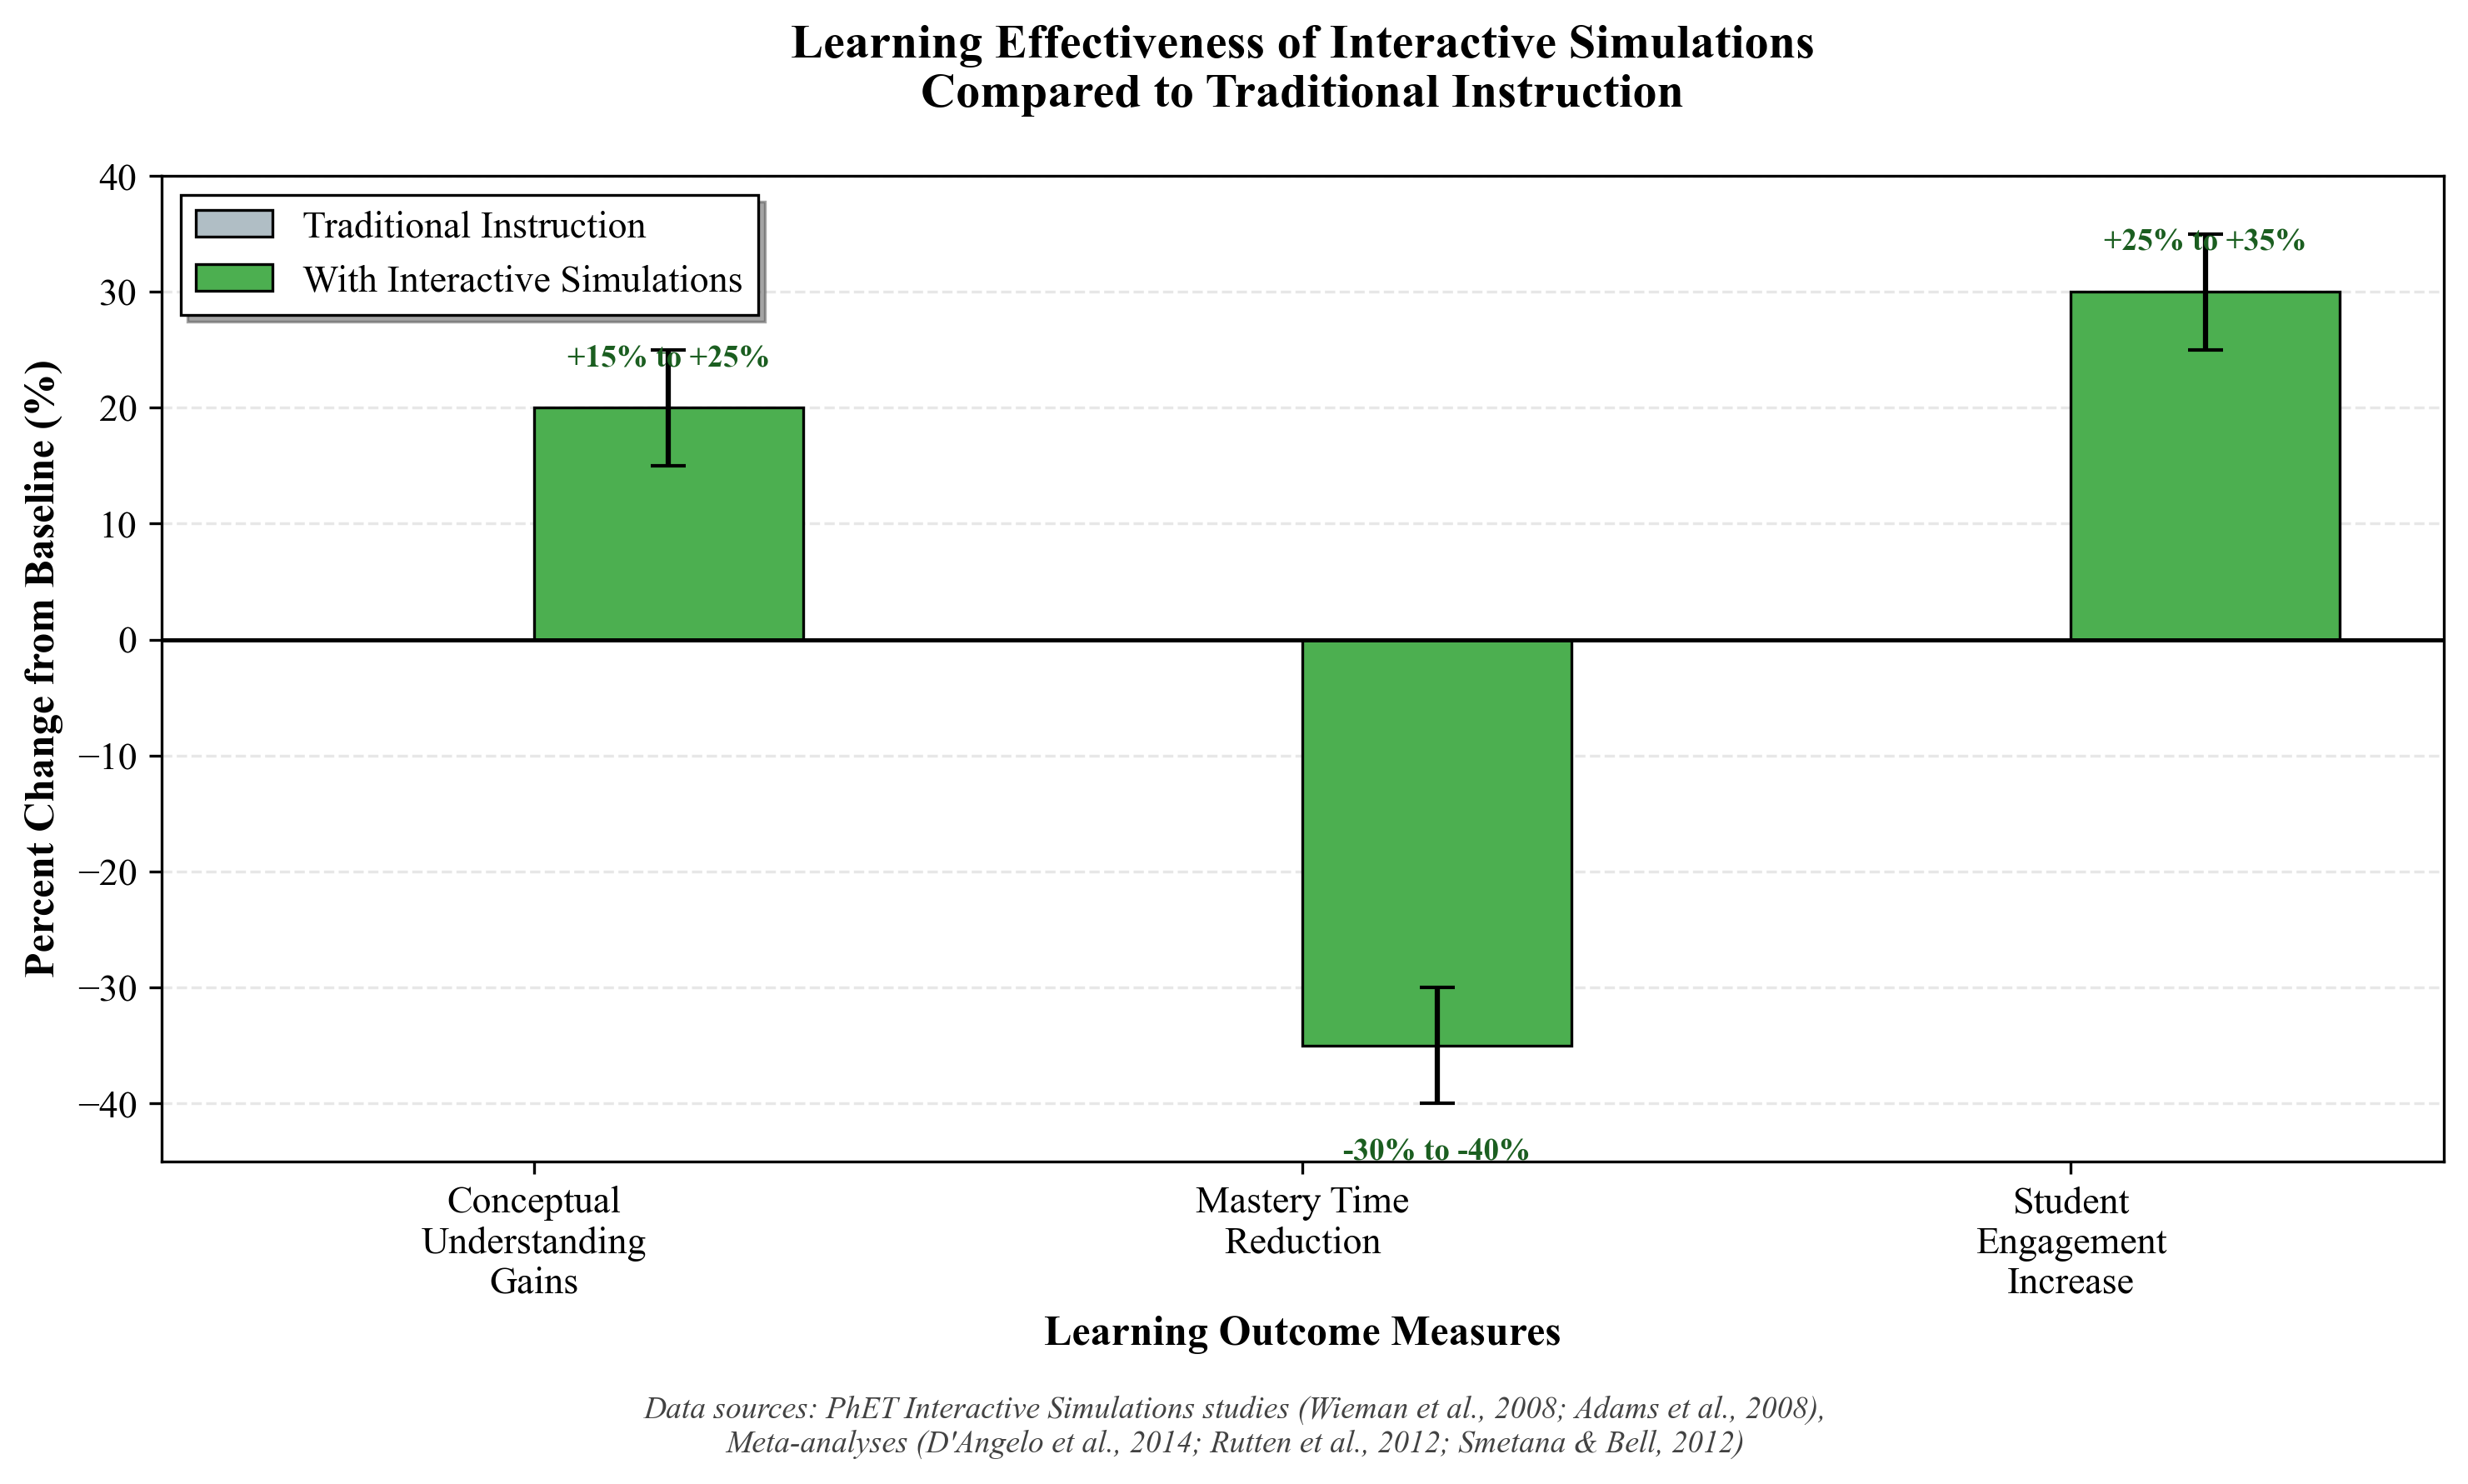
\includegraphics[width=0.95\textwidth]{figures/effectiveness-chart.png}
\caption{Learning effectiveness of interactive simulations compared to traditional instruction across three key outcome measures. Data represent meta-analysis findings from multiple studies including PhET Interactive Simulations research and systematic reviews across STEM disciplines. Error bars indicate reported ranges of improvement. Sources: Wieman et al. (2008), Adams et al. (2008), D'Angelo et al. (2014), Rutten et al. (2012), Smetana \& Bell (2012).}
\label{fig:effectiveness}
\end{figure}

These impressive gains, visualized in Figure~\ref{fig:effectiveness}, reflect simulations' ability to make abstract concepts tangible and provide immediate, interactive feedback that supports active learning. By allowing learners to \textit{visualize invisible processes} such as magnetic fields, molecular motions, or electric currents, simulations bridge the gap between theoretical knowledge and real-world phenomena \cite{phet2023}.

\subsection{PhET Interactive Simulations: Evidence at Scale}

The PhET Interactive Simulations project at the University of Colorado Boulder provides the most comprehensive evidence for simulation effectiveness at scale. With over 45 million simulation runs annually across 175 countries, PhET represents one of the largest deployments of educational simulations worldwide \cite{phet2023}. This massive usage scale, combined with extensive research validation, demonstrates both the practical feasibility and educational effectiveness of well-designed interactive simulations.

Studies of PhET simulations have demonstrated significant learning gains across diverse populations and educational contexts \cite{adams2008study, finkelstein2005phet, perkins2006phet}. In controlled experiments comparing simulation-based instruction to traditional approaches, students using PhET simulations consistently achieved higher scores on conceptual assessments and demonstrated superior long-term retention.

\textbf{Controlled Experimental Evidence}: In a particularly compelling controlled study, high school physics students were randomly assigned to learn circuit concepts using either PhET Circuit Construction Kit simulations or physical circuit equipment (wires, bulbs, resistors). Despite equivalent instructional time and support, students using the simulation significantly outperformed their peers who used physical equipment on subsequent conceptual exam questions. Most remarkably, six weeks after the initial instruction, the simulation group demonstrated substantially better knowledge retention, suggesting that the interactive visual feedback provided by the simulation created more durable mental models \cite{finkelstein2005phet}.

\textbf{Transfer to Physical Skills}: Perhaps most surprising, when both groups were eventually asked to construct physical circuits with real equipment, students initially trained on simulations performed the task faster and with greater confidence than those who had originally used physical apparatus. This finding challenges the common assumption that virtual experiences cannot adequately prepare students for hands-on tasks, instead suggesting that well-designed simulations can provide superior conceptual foundations that transfer effectively to practical applications \cite{finkelstein2005phet}.

\textbf{Classroom Implementation Patterns}: Survey research with hundreds of PhET-using educators reveals that teachers employ simulations flexibly across diverse pedagogical contexts: demonstrations during lectures, guided inquiry laboratory activities, homework assignments, and remediation for struggling students. The primary goals educators report for using simulations include developing conceptual understanding, promoting scientific inquiry skills, and addressing known misconceptions \cite{phet2023}.

\subsection{How Students Interact with MicroSims}

Understanding how students actually engage with interactive simulations illuminates why these tools prove effective and what design principles support productive learning interactions. Research based on classroom observations, student interviews, and interaction logging provides detailed insights into the phenomenology of simulation-based learning.

\subsubsection{Guided Exploration and Playful Experimentation}

Students typically interact with effective simulations through a combination of guided exploration and playful experimentation. Well-designed simulations employ \textit{intuitive interfaces} with minimal text requirements, familiar object representations, and direct manipulation controls that enable learners of various ages to begin exploring immediately. PhET simulations exemplify this design philosophy by using everyday objects such as light bulbs, beakers, and bicycles as interface icons, helping students connect scientific concepts to prior knowledge and lived experience \cite{phet2023}.

As students manipulate simulation parameters through sliders, buttons, and direct object manipulation, the simulation provides instant animated feedback that makes cause-and-effect relationships immediately visible. This interactivity invites learners to pose "What if..." questions and observe consequences in real time, fostering hypothesis generation and empirical testing behaviors characteristic of scientific thinking.

Classroom observations reveal a distinctive interaction pattern: students often engage in initial playful exploration, manipulating controls with apparent randomness, then gradually focus attention on underlying scientific principles as they notice systematic patterns and regularities. This progression from play to focused inquiry appears to be pedagogically productive, as the initial exploratory phase builds familiarity with the simulation interface and generates questions that motivate subsequent systematic investigation \cite{phet2023}.

\subsubsection{The Critical Role of Scaffolding}

The level of instructional guidance accompanying simulations significantly influences the depth and quality of student engagement. Research comparing different activity structures reveals that both extremes—highly prescriptive step-by-step procedures and completely unguided free exploration—produce suboptimal learning outcomes \cite{phet2023}.

Overly structured activities that specify every action and observation lead to shallow, procedure-following behavior where students complete tasks without developing genuine conceptual understanding. Students in such contexts often focus on obtaining the "correct answer" rather than exploring the underlying phenomena or constructing their own understanding.

Conversely, completely unguided exploration can leave students overwhelmed by the simulation's possibility space, uncertain what aspects merit attention, and unable to connect their observations to relevant scientific principles. Without some strategic direction, many students may never discover the simulation's most pedagogically significant features or recognize the conceptual importance of particular phenomena.

The optimal approach identified by research provides \textit{minimal but strategic scaffolding}: a few well-designed open-ended questions or challenges that guide students toward investigating key features without dictating specific procedures. Such "gentle guidance" prompts might ask students to "find three ways to make the bulb brighter" or "predict what will happen when you double the voltage, then test your prediction" \cite{phet2023}.

This balanced scaffolding approach encourages self-directed inquiry where students form predictions, design tests, observe outcomes, and refine their understanding through iterative cycles. Students engaging in this guided-but-not-prescribed exploration demonstrate deeper conceptual reasoning than peers experiencing either overly structured or completely unstructured activities \cite{phet2023}.

\subsubsection{Collaborative Learning and Peer Discussion}

Classroom implementations frequently position simulations as collaborative activities where students work in pairs or small groups. This social configuration promotes productive peer discussion as students debate predictions, explain observations to one another, and collectively make sense of simulation behaviors. The collaborative context transforms individual cognitive engagement into social knowledge construction, with students challenging each other's misconceptions and collectively building more sophisticated understanding.

The simulations' visual, dynamic nature provides a shared referent for group discussion—students can point to specific elements on screen, propose interpretations of what they observe, and negotiate meaning through dialogue anchored in their common perceptual experience. This shared visual reference appears to scaffold productive scientific argumentation even among younger learners who might struggle with purely verbal scientific discourse.

\subsubsection{Safe Experimentation and Risk-Taking}

A consistently reported benefit of simulation-based learning is that virtual environments eliminate risks associated with physical experimentation. Students demonstrate greater willingness to try unconventional approaches, test extreme parameter values, and recover from "failures" when working with simulations compared to physical equipment \cite{phet2023}.

One revealing study contrasted students' affective responses when using circuit simulations versus real circuit equipment. Students working with physical apparatus expressed nervousness about breaking expensive equipment or injuring themselves, leading to cautious, conservative exploration strategies. In contrast, students using the Circuit Construction Kit simulation "explored and investigated without needing much assistance," trying diverse configurations and learning through trial and error without anxiety about consequences \cite{finkelstein2005phet}.

This psychological safety appears particularly valuable for students from groups traditionally underrepresented in STEM fields, who may experience heightened anxiety about appearing incompetent or damaging equipment. By removing performance pressure and material consequences, simulations can provide more equitable access to exploratory learning experiences.

\subsection{Effectiveness Across Grade Levels}

One of the most significant advantages of well-designed interactive simulations is their pedagogical effectiveness across diverse educational levels, from upper elementary school through higher education. This adaptability enables the same fundamental design principles to support age-appropriate learning across a remarkably wide developmental span.

\subsubsection{Elementary Education (Grades 3-5)}

Research demonstrates that even young learners aged 10-12 can benefit substantially from appropriately designed simulations. In one longitudinal study, fifth and sixth grade students used an ecosystem simulation over multiple class sessions and demonstrated "considerable improvements" in systems thinking skills, including understanding of ecological processes and interactions \cite{eric2009}. This evidence challenges assumptions that complex system modeling exceeds young learners' capacities, suggesting instead that well-designed simulations can scaffold sophisticated thinking even in elementary contexts.

Effective simulations for this age group employ simpler interfaces, more scaffolding guidance, and contexts tied to students' everyday experiences. Visual design typically employs cartoon-style graphics and anthropomorphized representations that appeal to younger learners while maintaining scientific accuracy. The content focus remains on foundational concepts presented through familiar scenarios—for example, exploring food webs through animals students recognize, or investigating basic physics through playground equipment simulations.

Despite the relative scarcity of research on elementary-level simulation use, existing evidence suggests substantial potential impact. As one systematic review noted, this scarcity represents a significant gap and opportunity: developing more MicroSims targeting K-5 curriculum standards could yield considerable benefits, particularly for schools lacking hands-on science resources \cite{mdpi2024}.

\subsubsection{Middle School (Grades 6-8)}

Middle school students, with their developing capacity for abstract reasoning, readily engage with simulations addressing introductory physics, earth science, pre-algebra, and life science topics. This developmental stage represents an optimal window for simulation-based instruction, as students can handle moderately complex interfaces while still benefiting from visual, interactive representations of abstract concepts.

Research at this level demonstrates simulations' effectiveness for addressing common misconceptions that emerge as students begin formal study of scientific phenomena. For example, simulations addressing force and motion help students overcome prevalent Aristotelian misconceptions about objects in motion, while chemistry simulations addressing particulate models of matter challenge students' intuitive but incorrect ideas about dissolving and chemical reactions.

\subsubsection{High School (Grades 9-12)}

At the high school level, simulations become integral components of rigorous STEM courses. Physics, chemistry, and biology courses routinely employ simulations both as alternatives to physical laboratory experiments and as unique learning tools that enable investigations impossible with physical equipment. Survey research reveals that high school and college instructors often use identical PhET simulations but adapt the surrounding activities and expectations to match student developmental levels \cite{phet2023}.

High school simulations can incorporate quantitative analysis, complex parameter spaces, and open-ended investigation designs that challenge advanced students while remaining accessible through intuitive visual interfaces. Students at this level increasingly use simulations for homework and independent study, indicating that well-designed tools can support self-directed learning outside formal classroom contexts.

\subsubsection{Higher Education}

At the college and university level, simulations support sophisticated conceptual understanding in introductory courses while also serving specialized functions in advanced coursework. In large-enrollment introductory courses, simulations provide active learning experiences that would be logistically impossible with physical equipment given typical class sizes and resource constraints.

For more advanced courses, simulations enable exploration of phenomena that would require specialized, expensive equipment (such as quantum mechanical systems or high-energy particle interactions) or dangerous procedures (such as chemical reactions involving hazardous materials). Graduate-level simulations may incorporate research-grade models and extensive parameter customization, blurring the boundary between educational tools and research instruments.

\textbf{Summary Across Levels}: While specific implementations vary by educational level, several core benefits remain consistent across all age groups: simulations make learning interactive and visual, provide immediate feedback, enable safe experimentation, and transform abstract concepts into manipulable experiences. The primary differences involve interface complexity, conceptual sophistication, and the degree of instructional scaffolding provided. This developmental continuity suggests that establishing simulation literacy early—through elementary and middle school experiences—prepares students to leverage increasingly sophisticated simulation-based learning as they advance through their education.

\subsection{Common Characteristics of Effective MicroSims}

Research on simulation effectiveness identifies several key design characteristics that consistently correlate with improved learning outcomes. These characteristics should inform development of new educational simulations and provide evaluation criteria for assessing existing resources.

\textbf{Intuitive, Student-Friendly Interfaces}: Effective simulations employ clean visual designs, minimal text requirements, and familiar metaphors that enable students to begin productive exploration without extensive instruction. Controls utilize standard interaction paradigms (dragging, sliding, clicking) and respond instantly, creating smooth dialogues between student actions and simulation feedback \cite{phet2023}. Intuitive design minimizes extraneous cognitive load, allowing learners to focus mental resources on scientific content rather than interface navigation.

\textbf{Familiar Contexts and Analogies}: The most pedagogically effective simulations depict scenarios or objects that students recognize from everyday experience: bicycles, balloons, magnets, kitchen utensils. This contextualization in familiar situations helps students activate relevant prior knowledge and form connections between scientific principles and lived experience \cite{phet2023}. Analogies embedded within simulations—such as modeling electric current flow using water flow—further aid conceptual understanding by connecting unfamiliar scientific phenomena to more intuitive physical systems.

\textbf{Making the Invisible Visible}: Perhaps the most distinctive pedagogical affordance of interactive simulations is their capacity to visualize normally invisible processes. Effective simulations render visible the phenomena students must understand but cannot directly observe: electrons moving through circuits, molecules colliding during chemical reactions, magnetic fields extending through space, quantum wave functions evolving over time \cite{phet2023, finkelstein2005phet}.

Many high-quality simulations provide multiple linked representations—for example, showing both a macroscopic view of a chemical reaction and a molecular-level animation simultaneously, or coordinating a physical simulation with real-time graphical plots of relevant variables. These coordinated representations help students construct connections between different levels of analysis and develop more integrated understanding \cite{phet2023}.

\textbf{Interactive and Responsive Feedback}: High-quality simulations provide immediate, dynamic responses to every student action. When learners adjust a slider, add an object, or change a parameter value, the simulation responds instantly with animated changes, updated graphs, and modified outcomes. This immediacy reinforces cause-and-effect relationships and supports learning through exploration and experimentation \cite{phet2023}.

Effective simulations also incorporate productive constraints—boundaries on possible actions that focus attention on scientifically relevant phenomena without overtly prescribing student behavior. For example, a circuit simulation might physically prevent impossible connections while allowing all valid circuit configurations, subtly guiding students toward productive exploration without explicitly instructing them what to try.

\textbf{Appropriate Challenge and Scaffolding}: The most effective simulations achieve a careful balance between ease of use and intellectual challenge. They often include implicit puzzles or goal-oriented tasks—such as achieving a stable orbit in a gravity simulation or lighting a bulb with limited circuit components—that spark curiosity and motivate exploration \cite{phet2023}.

Simultaneously, simulations must remain accessible through intuitive controls and clear visual feedback that prevent frustration. Many successful simulations accompany their open-ended design with optional hints, guiding questions, or progressive complexity levels that provide scaffolding for struggling students while remaining unobtrusive for those who prefer independent exploration.

\textbf{Research-Tested and Refined}: A distinguishing feature of the most effective educational simulations is that they undergo extensive iterative testing and refinement driven by education research. PhET simulations exemplify this approach, with each simulation progressing through multiple development cycles involving student interviews, classroom observations, and systematic assessment of learning outcomes \cite{phet2023}.

This research-based refinement process results in simulations that effectively target known misconceptions, provide intuitive interfaces that align with student thinking, and include design features specifically engineered to promote correct conceptual understanding. The documented effectiveness of research-tested simulations underscores the importance of evidence-based design processes rather than relying solely on designer intuition or general software engineering principles.

\subsection{High-Impact Application Categories}

Based on extensive research and documented effectiveness, several categories of interactive simulations emerge as particularly high-impact for STEM education. These domains represent areas where simulations provide unique pedagogical value and where continued development efforts promise substantial educational returns.

\subsubsection{Physics and Engineering}

Physics has proven extraordinarily fertile ground for educational simulations, given the field's abstract concepts and often-invisible forces. Simulations covering classical mechanics (motion, gravity, energy conservation), electromagnetism (circuits, fields, magnetism), waves (sound, light, interference), and modern physics (quantum phenomena, relativity) have demonstrated consistently strong impacts on student learning \cite{wieman2008phet, finkelstein2005phet}.

Physics simulations enable students to visualize forces and fields, manipulate time scales to slow motion or observe long-term system evolution, and experiment with parameter values impossible to achieve or isolate in physical laboratory settings. Circuit simulations, for example, allow students to observe charge flow directly and instantly reconfigure connections, leading to superior conceptual understanding compared to using physical wires and components \cite{finkelstein2005phet}.

Engineering-oriented simulations provide sandbox environments for design and experimentation, enabling students to construct bridges, design electrical systems, or optimize mechanical devices through iterative testing without material costs or safety concerns. These simulations develop both domain knowledge and design thinking skills essential for engineering practice.

Future development priorities in this category include simulations for advanced topics that are particularly difficult to demonstrate in traditional classrooms: magnetic field interactions, semiconductor physics, relativistic effects, and quantum mechanics visualizations. Such simulations could make typically abstract and mathematically intensive content more accessible and intuitive for broader student populations.

\subsubsection{Chemistry and Molecular Science}

Chemistry simulations possess unique power to transport students into the molecular realm, making visible the atomic and molecular processes underlying macroscopic chemical phenomena. High-impact examples address chemical bonding, reaction mechanisms, equilibria, gas laws, solutions and pH, and atomic structure \cite{phet2023}.

Effective chemistry simulations typically feature multiple coordinated representations: molecular animations showing individual particles alongside macroscopic views and graphical plots of concentration, energy, or other relevant variables. These linked representations help students construct connections between molecular behaviors and observable chemical properties—a notoriously difficult conceptual leap in chemistry education \cite{phet2023}.

Chemistry simulations also provide virtual laboratory environments for experiments that would be dangerous, expensive, or time-consuming with physical materials. Students can explore reaction kinetics by instantly adjusting temperature or try numerous reactant combinations without safety concerns or material costs. The ability to observe molecular collision dynamics and reaction mechanisms provides insights impossible to achieve through physical laboratory work.

Research indicates that molecular-level simulations effectively address common misconceptions about dissolving, phase changes, and chemical reactions while improving overall conceptual understanding in chemistry courses \cite{mdpi2024}. Developing additional simulations for under-represented topics such as organic reaction mechanisms, electrochemistry, and environmental chemistry processes could substantially enhance chemistry education accessibility and effectiveness.

\subsubsection{Biology and Life Sciences}

In biological sciences, simulations model processes occurring within organisms and ecosystems, often involving time scales and spatial scales difficult to observe directly. Cell and molecular biology simulations addressing gene expression, cellular respiration, and protein synthesis enable students to manipulate biological pathways and observe consequences, supporting understanding of complex biochemical sequences \cite{mdpi2024}.

Human anatomy and physiology simulations provide interactive models of body systems—circulatory, nervous, digestive—that are more ethical and often more informative than traditional dissection while remaining highly engaging for students. The ability to highlight specific components, show invisible processes like nerve signal transmission, and manipulate physiological parameters provides learning experiences impossible through physical specimens.

At larger scales, ecology and environmental science simulations model population dynamics, predator-prey relationships, disease transmission, and climate systems. These simulations allow students to experiment with ecological parameters and observe long-term consequences in accelerated time, promoting systems thinking by revealing how changes in one system component cascade through interconnected networks \cite{eric2009}.

One elementary-level study using an ecosystem simulation found substantial improvements in students' systems thinking skills, including understanding of processes, interactions, and ecological relationships. However, the study also identified persistent difficulties with feedback loops and cyclical causation, suggesting that further simulation design innovation is needed to effectively scaffold understanding of these complex system dynamics \cite{eric2009}.

Biology simulations prove particularly engaging because they connect to personally relevant topics—health, environment, organisms students encounter—and often incorporate game-like scenarios such as maintaining ecological balance or preventing disease outbreaks. Expanding simulation resources for genetics, evolution, microbiology, and complex ecosystem modeling represents a high-priority development area likely to yield significant educational impact.

\subsubsection{Mathematics and Computational Thinking}

Mathematics-focused simulations help students visualize abstract mathematical concepts by transforming them into interactive, manipulable objects. Examples span from elementary-level simulations exploring fractions through adjustable visual representations to advanced mathematics involving function transformations, multivariable calculus, and linear algebra.

Algebra and geometry simulations enable learners to manipulate equations or geometric objects and immediately observe resulting changes, reinforcing concepts such as slope, transformations, congruence, and similarity through dynamic visual feedback. Probability and statistics simulations allow students to conduct virtual experiments with thousands of trials in seconds, building intuition about randomness, sampling distributions, and statistical inference that would be impractical to develop through physical experiments.

While mathematics simulations have received less research attention than science simulations, platforms including PhET offer numerous mathematics-focused tools, and educator reports indicate positive impacts on engagement and conceptual understanding. Connecting mathematical concepts to visual, manipulable representations appears particularly beneficial for students who struggle with purely symbolic mathematical notation.

Computational thinking and computer science concepts can also be taught through carefully designed simulations: guiding virtual robots through mazes to teach programming logic, visualizing sorting algorithms, or manipulating data structures. As computational thinking becomes increasingly central to K-12 curricula, simulation-based approaches offer accessible entry points for students without prior programming experience.

Future development priorities include simulations for calculus concepts (such as interactive integral visualization accumulating area), linear algebra (visualizing vector spaces and matrix transformations), and applied mathematics contexts (financial modeling, engineering applications) that demonstrate real-world relevance while building mathematical understanding.

\subsubsection{Complex Systems and Systems Thinking}

This cross-disciplinary category addresses one of education's most significant challenges: developing students' capacity to understand complex, dynamic systems with multiple interconnected components. Systems thinking simulations model phenomena characterized by feedback loops, time delays, emergent behaviors, and non-obvious cause-effect relationships \cite{eric2009}.

Examples include environmental systems (climate models, water resource management), socio-economic systems (urban development, economic models), and integrated science issues (energy grids combining physics, economics, and environmental factors). Such simulations allow students to manipulate system components and observe cascading effects, teaching them to think in terms of stocks, flows, delays, and feedback loops rather than simple linear causation.

Research with ecosystem simulations for middle school students demonstrated improvements in understanding system structures and component interactions, but also revealed persistent difficulties with feedback loops and cyclical causation \cite{eric2009}. These findings suggest both the promise and challenge of systems thinking education: simulations can effectively scaffold certain aspects of systems thinking, but current designs may require enhancement to adequately address the most conceptually difficult elements of complex systems.

High-impact systems simulations effectively visualize flows of conserved quantities (energy, matter, money, population) and accumulate changes over time through graphical displays. They encourage what-if analysis, positioning students as decision-makers exploring policy consequences: "What happens if we increase recycling rates by 50\%? What if we introduce a new predator species?"

Causal loop diagrams, stock-and-flow models, and system dynamics simulations help students recognize circular causation, time delays, and system equilibria—essential concepts for understanding global challenges involving climate, resources, public health, and social systems. Given the importance of systems thinking for addressing complex real-world problems, continued development of accessible, pedagogically effective simulations in this category represents a high-priority investment likely to yield substantial educational and societal returns.

\subsection{Subject Areas Requiring Specialized Supporting Libraries}

While p5.js provides an excellent foundation for many educational simulations, certain subject areas require specialized visualization or interaction libraries to achieve maximal pedagogical effectiveness. Identifying these areas and developing appropriate supporting libraries represents an important priority for expanding MicroSim capabilities across the full curriculum.

\subsubsection{History and Geography}

Historical and geographical education benefit tremendously from timeline and mapping visualizations that contextualize events spatially and temporally. However, creating effective interactive timelines and geographic visualizations requires specialized libraries beyond p5.js core capabilities.

\textbf{Timeline Visualizations}: Libraries such as vis-timeline.js enable creation of interactive historical timelines where students can explore event sequences, understand historical periods, and recognize concurrent developments across different regions or domains. Educational applications include comparing technological developments across civilizations, understanding cause-and-effect sequences in historical events, and recognizing patterns in historical change. High-quality timeline templates incorporating pedagogical best practices would significantly lower barriers to creating history-focused MicroSims.

\textbf{Geographic Mapping}: Libraries like Leaflet.js provide interactive mapping capabilities essential for geography, environmental science, and social studies education. Geographic simulations could enable students to explore resource distribution, understand migration patterns, investigate environmental changes, or analyze geopolitical relationships. Integrating mapping libraries with MicroSim design patterns while maintaining the framework's simplicity and generative AI compatibility represents an important technical challenge with substantial educational payoff.

\subsubsection{Electrical Circuits and Signal Processing}

Circuit education presents unique challenges requiring specialized component libraries for drawing schematic diagrams, simulating circuit behavior, and animating current flow. While PhET's Circuit Construction Kit demonstrates the pedagogical value of interactive circuit simulations, creating new circuit simulations currently requires substantial specialized programming.

\textbf{Circuit Schematic Components}: A comprehensive p5.js circuit drawing library providing standard electrical components (resistors, capacitors, batteries, switches, transistors) with appropriate connection logic would enable rapid development of circuit-focused MicroSims. Such a library should handle component placement, connection validation, and visual rendering while exposing circuit state for educational visualization.

\textbf{Current Animation}: Animating electron flow or current direction provides crucial visual feedback for understanding circuit behavior. A supporting library providing current animation capabilities—showing moving charges, indicating direction, and responding to circuit modifications—would substantially enhance circuit simulation pedagogical effectiveness.

\textbf{Signal Processing}: Related applications in signal processing, communications, and electrical engineering would benefit from libraries supporting waveform visualization, frequency analysis, and filter design. Enabling students to interactively explore Fourier analysis, modulation schemes, or digital signal processing through well-designed simulations could significantly improve accessibility of these mathematically intensive topics.

\subsubsection{Systems Dynamics and Causal Loop Diagrams}

Teaching systems thinking benefits from specialized visualization tools for stock-and-flow diagrams and causal loop diagrams. These representations help students understand accumulation, feedback loops, and circular causation in complex systems \cite{eric2009}.

A library supporting creation and interactive manipulation of causal loop diagrams would enable students to construct, test, and refine their own system models, promoting deeper engagement with systems thinking concepts. Such a library should support standard systems dynamics notation while remaining accessible for middle school through university students.

\subsection{Limitations and Challenges}

Despite their demonstrated effectiveness, educational simulations face several important limitations and challenges that must be acknowledged and addressed through ongoing research and development.

\textbf{Scope Constraints}: The deliberately focused nature of MicroSims means individual simulations cannot address all learning objectives within a domain. Complex, multi-faceted concepts may require sequences of simulations or complementary instructional approaches. Educators must thoughtfully integrate simulations within broader curriculum frameworks rather than viewing them as comprehensive, standalone educational solutions.

\textbf{Abstraction and Simplification}: By necessity, simulations simplify reality to make phenomena comprehensible and computable. While these simplifications often serve legitimate pedagogical purposes, they risk creating misconceptions if students do not understand model limitations. Simulations should explicitly document their assumptions and help students recognize that models are useful approximations rather than complete representations of reality.

\textbf{Technology Access and Digital Divide}: While browser-based simulations reduce technology barriers compared to specialized software, they still require reliable internet access and functional computing devices. Socioeconomic disparities in technology access risk making simulation-based learning another dimension of educational inequality unless intentionally addressed through school technology provisioning and alternative access strategies.

\textbf{Quality Variability}: Not all simulations prove equally effective. Poorly designed simulations can confuse rather than clarify, promote misconceptions, or simply fail to engage students productively. The demonstrated success of research-tested simulations like PhET underscores the importance of evidence-based design and iterative refinement. However, the MicroSims framework's goal of enabling rapid AI-assisted generation introduces quality assurance challenges requiring systematic approaches to validation and improvement.

\textbf{Teacher Preparation and Support}: Effective simulation use requires thoughtful pedagogical integration. Teachers need support in selecting appropriate simulations, designing accompanying activities with optimal scaffolding levels, and facilitating productive classroom discussions around simulation experiences. Professional development and high-quality instructional materials represent essential infrastructure for realizing simulations' educational potential.

\textbf{Assessment Integration}: Evaluating learning from simulation experiences presents ongoing challenges. While simulations generate rich interaction data potentially valuable for formative assessment, translating simulation performance into meaningful learning evaluation remains underdeveloped. Embedding meaningful assessment within simulations while maintaining their lightweight character requires continued innovation.

\subsection{Intelligent Textbook Integration Example}

The MicroSims framework envisions simulations not as isolated educational resources but as integrated components of intelligent, adaptive learning systems. An intelligent textbook system demonstrates how simulations can function within broader educational ecosystems to provide personalized, data-driven learning experiences.

\textbf{Adaptive Content Sequencing}: An intelligent textbook incorporating MicroSims continuously assesses student understanding through interaction patterns, simulation performance, and embedded assessment items. Based on this ongoing evaluation, the system adaptively sequences content—determining when students have sufficiently mastered prerequisites to advance, when additional practice through simulation exploration would benefit learning, or when remediation through alternative representations might address persistent misconceptions.

\textbf{Personalized Simulation Selection}: Rather than presenting identical content to all students, an intelligent textbook can select from libraries of related simulations targeting the same concepts at different complexity levels or through different contextual framings. A student struggling with abstract mathematical representations might receive a simulation emphasizing concrete, everyday contexts, while an advanced student might encounter more sophisticated parameter spaces and quantitative analysis tasks.

\textbf{Learning Analytics and Feedback Loops}: Comprehensive logging of student interactions with embedded simulations—including time spent, parameters explored, challenges attempted, and errors made—provides rich data for learning analytics. Intelligent systems analyze these data streams to identify struggling students requiring intervention, recognize common misconceptions requiring instructional attention, and refine content recommendations based on observed effectiveness patterns.

\textbf{Integration with Reinforcement Learning}: Advanced implementations might employ reinforcement learning algorithms that treat simulation selection and sequencing as optimization problems: the system learns through trial and error which combinations of simulations, scaffolding levels, and timing produce optimal learning outcomes for different student profiles. Over time, such systems become increasingly effective at personalizing educational experiences as they accumulate data about what works for whom under what circumstances.

This vision of intelligent textbook integration positions MicroSims as essential building blocks for next-generation adaptive learning systems—systems that combine the engagement and interactivity of simulations with the personalization and continuous improvement capabilities of AI-driven education technology.
